\begin{wrapfigure}{r}{0.35\textwidth}
    \centering
    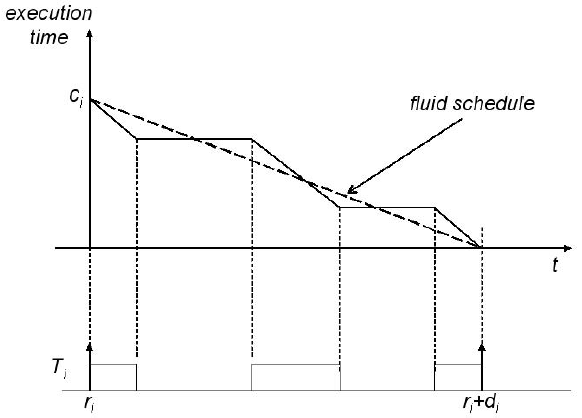
\includegraphics[width=0.35\textwidth]{figure-1}
    \caption{\emph{Fluid Schedule} vs \emph{Practical Schedule}}
    \label{fig:figure-1}
\end{wrapfigure}

\paragraph{\textnormal{\textbf{LLREF Scheduling Algorithm}}} \underline{The Model:} Se considera \emph{global scheduling}, en donde la migración de tareas no está restringuidas,  en un systema \emph{Symmetric Multi-Processor} (SMP) con $M$ procesadores idénticos. Se considera que la aplicación consiste de un conjunto de tareas denotadas con \textbf{T=}$\{T_1, T_2, \dots, T_N\}$. Se asume que las tareas arriban periódicamente en sus \emph{release times} $r_i$. Cada tarea $T_i$ tiene un tiempo de ejecución $c_i$, y un \emph{deadline} relativo $d_i$ el cual es el mismo que su periódo $p_i$. La utilización $u_i$ de una tarea $T_i$ se define como $c_i/d_i$ y se asume que es menor a 1. Se asume que las tareas puede ser rechazadas en cualquier momento y que son independientes. Se considera una política no conservadora de trabajo, por esto los procesadores pueden estar inactivos incluso cuando las tareas están presenten en la cola de \emph{ready}.


\underline{Time and Local Execution Time Plane:} en el modelo \emph{fluid scheduling}, cada tarea se ejecuta en una tasa constante en todo momento. En el modelo de este algoritmo de \emph{scheduling} se consideraron el modelo \emph{fluid scheduling} y la noción de equidad (\emph{fairness}). Se considera una abstracción llamada \emph{Time and Local Execution Time Domain Plane (T-L plane}), en donde las tareas se representan como \emph{tokens} que se mueven en el tiempo. Se usa \emph{T-L plane} para describir \emph{fluid schedules} y se presenta un nuevo algoritmo de \emph{scheduling} que está en la capacidad de rastrear el \emph{fluid schedule} sin utilizar datos de quantum.  


\begin{wrapfigure}{l}{0.34\textwidth}
    \centering
    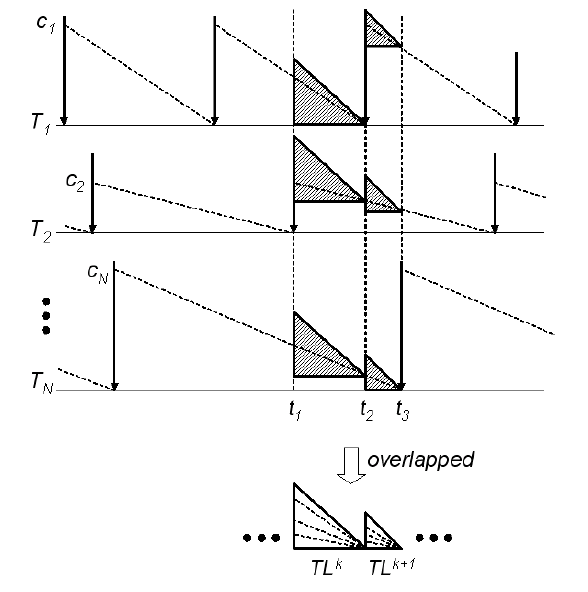
\includegraphics[width=0.34\textwidth]{figure-2}
    \caption{T-L Planes}
    \label{fig:figure-2}
\end{wrapfigure}

Para una tarea $T_i$, con $r_i, c_i$ y $d_i$ la Figura \ref{fig:figure-1}  muestra un plano bidimensional con el tiempo representado en el eje $x$ y el tiempo de ejecución restante de una tare en el eje $y$. Si $r_i$ se asume como el origen, la línea punteada desde $(0, c_i)$ a $(d_i, 0)$ indica el \emph{fluid schedule}, cuya pendiente es $u_i$. Debido que el \emph{fluid schedule} es ideal pero practicamente imposible, la equidad de un algoritmo de \emph{schedule} depende en qué tanto el algoritmo se aproxime a la ruta del \emph{fluid schedule}. Cuando $T_i$ corre como en la Figura \ref{fig:figure-1}, su ejecución puede ser representada como una línea discontinua entre $(0, c_i)$ y $(d_i, 0)$. Nótese que la ejecución de la tarea se representa como una línea cuya pendiente es -1, debido a que los vértices $x$ y $y$ están en la misma escala y la no-ejecución en el tiempo se representa como una línea cuya pendiente es cero. Cuando $N$ número de tareas son consideradas, sus \emph{fluid schedules} pueden ser construidos como en la Figura \ref{fig:figure-2} y para cada tarea se puede encontrar un un triángulo isósceles a la derecha entre cada dos eventos de \emph{scheduling} consecutivos y $N$ triángulos entre cada dos eventos de \emph{scheduling} pueden ser sobrepuestos.   


A esto se le llama el \emph{T-L plane} $TL^k$, en donde $k$ simplemente incrementa con el tiempo. El tamaño de $TL^k$ puede cambiar en $k$. La parte de abajo del triángulo representa el tiempo. El lado izquierdo del triángulo representa el eje de una parte del tiempo de ejecución de las tareas restantes, al que se le llama \emph{local remaining execution time} $l_i$, que se supone que sea consumido antes que cada $TL^k$ finalice. \emph{Fluid schedules} para cada tarea pueden ser construidos como si estuvieran sobrepuestas en cada plano $TL^k$, mientras mantienen sus pendientes.
\underline{Scheduling in \emph{T-K plane}:} La abstracción del \emph{T-L plane} es significativa en \emph{scheduling} de multiprocesadores, porque los \emph{T-L planes} se repiten en el tiempo y un buen algoritmo de \emph{scheduling} para un solo \emph{T-L plane} está en la capacidad de planificar/programar tareas para todos los \emph{T-L planes} repetidos. Aquí, por buen algoritmo se quiere decir que este en la capacidad de construir una planificación que permita que la ejecución de todas las tareas en el \emph{T-L plane} se aproxime a el \emph{fluid schedule} tanto como sea posible. El estatus de cada tarea se representa como un \emph{token} en el \emph{T-L plane}. La localización del token describe el tiempo actual comoun valor en el eje horizontal y el tiempo de ejecución restante como un valor en el eje vertical. Aquí, el tiempo de ejecución restante de una tarea significa uno que deba ser consumido hasta el tiempo $t_{f}^{k}$ y no el \emph{deadline} de la tarea.
 
\begin{wrapfigure}{l}{0.35\textwidth}
    \centering
    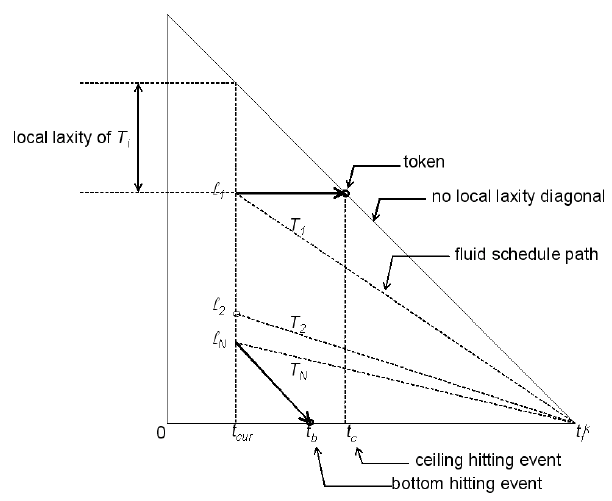
\includegraphics[width=0.35\textwidth]{figure-3}
    \caption{$k^{th}$ T-L Plane}
    \label{fig:figure-3}
\end{wrapfigure}

Como las decisiones de \emph{scheduling} se hacen en el tiempo, el token de cada tarea se mueve en el \emph{T-L plane}. Aunque las rutas ideales de un token existen como una línea punteada en la Figura \ref{fig:figure-3}, a los tokens solamente se les permite moverse en dos direcciones. Cuando la tarea se selecciona y se ejecuta, el token se mueve diagonalmente hacia abajo, conforme $T_N$ se mueve. De otra forma, se mueve horizontalmente, conforme $T_1$ se mueve. Si $M$ procesadores son considerados, a lo sumo $M$ tokens pueden moverse juntos en diagonal. El objectivo de \emph{scheduling} en el $k^{th}$ \emph{T-L plane} es hacer que todos los tokens arriben en el vértice más a la derecha del \emph{T-L plane}. A este arribo existoso se le llama factibilidad local. Si todos los tokens son localmente factibles en cada \emph{T-L plane}, es posible que sean planicables a través de cada \emph{T-L plane} consecutivo en el tiempo, aproximando todas las tareas a sus rutas ideales. Por conveniencia, se define el \emph{local laxity} de una tarea $T_i$ como $t_{f}^{k} - t_{cur} - l_i$, donde $t_{cur}$ es el tiempo actual. El lado oblicuo del \emph{T-L plane} tiene significado importante: cuando un token alcanza ese lado, implica que la tarea no tiene ningún \emph{local laxity}. Así, si no es seleccionada inmediatamente, entonces no puede satisfacer el objectivo de \emph{scheduling} de factibilidad local. A este lado oblicuo del \emph{T-L plane} se le llama \emph{no local laxity diagonal} (NLLD). Todos los tokens se suponen que están entre la línea horizontal y la diagonal de \emph{local laxity}. Se observa que hay dos instantes cuando las decisiones de \emph{scheduling} se tienen que hacer otra vez en el \emph{T-L plane}. Un instante es cuando el tiempo de ejecución restante de una tarea es completamente consumido, y debería de ser mejor para el sistema correr otra tarea en su lugar. Cuando esto ocurre, el token alcanza la línea horizontal, como $T_N$ lo hace en la figura \ref{fig:figure-3}. A esto se le llama \emph{bottom hitting event} (o evento B). El otro instante es cuando el \emph{local laxity} de una tarea se vuelve 0 del tal forma que la tarea debe ser seleccionada inmediatamente. Cuando esto ocurre, el token alcanza el NLLD, como $T_1$ lo hace en la figura \ref{fig:figure-3}. A esto se le llama el \emph{ceiling hitting event} (o evento C). Para proveer factilibilidad local, $M$ tareas del tiempo local más grande de ejecución son seleccionadas de primero (o LLREF) para cada evento secundario. A esto se le llama LLREF \emph{scheduling policy}. Nótese que la tarea que tiene tiempo local de ejecución restante en 0 (el token que yace en la línea inferior el \emph{T-L plane}) no se permite ser seleccionada, lo que hace que la política de \emph{scheduling} sea \emph{non work-conserving}. Los tokens para estas tareas son llamadas inactivas y las otras con tiempo de local de ejecución restante mayor a 0 son llamadas activas. En el tiempo $t_{f}^{k}$, el instante del evento para la liberación de la próxima tarea, el próximo \emph{T-L plane} $TL^{k + 1}$ inicia y el LLREF permanece válido. Así, el LLREF \emph{scheduling policy} is aplicado consistentemente a cada evento.

\paragraph{\textnormal{\textbf{Algorithm Properties}}} \underline{\emph{1. Critical Moment:}} Todos los tokens que flujen de izquierda a derecha. LLREF selecciona $M$ tokens a partir de $N$ tokens activos y estos fluyen diagonalmente hacia abajo. Por otro lado, las otras que no son seleccionadas, toman caminos/rutas horizontales. Cuando un evento C o B sucede, denotado con $t_j$ donde $0 < j < f$, LLREF se invoca para realizar una decisión de \emph{scheduling}. Se define la utlización local $r_{i,j}$ para una tarea $T_i$ en el tiempo $t_j$ como $\frac{l_{i,j}}{t_f - t_j}$, lo que describe qué tanta capacidad de procesador necesita ser utilizado para ejecutar $T_i$ dentro del tiempo restante hasta $t_f$. Aquí, $l_{i,j}$ es el tiempo local de ejecución restante de la tarea $T_i$ en el tiempo $t_j$. Cuando $k$ se omite, implícitamente significa el $k-$ésimo \emph{T-L plane}. \underline{Teorema:} (Valor de utilización local inicial en el \emph{T-L plane}) Dejar que todos los tokens arriben al vértice más a la derecha en el $(k - 1)^{(th)}$ \emph{T-L plane}. Entonces, el valor de utilización local inicial $r_{i,0} = u_i$ para todas las tareas $T_i$ en el $(k - 1)^{(th)}$ \emph{T-L plane}. Se define el momento crítico para describir la condición necesaria y suficiente que todos los tokens no son localmente factibles (factibilidad local de los tokens implica que todos los tokesn no arriban simultaneamente al vértice más a la derecha del \emph{T-L plane.} El momento crítico es el primer evento secundario en que más de $M$ tokens alcanzan simultaneamente NLLD. \underline{Teorema:} (Critical moment)  Como mínimo un momento crítico ocurre si y solo si los tokens no soy localmente factibles en el \emph{T-L plane}. 

\underline{Evento C:} El evento C pasa cuando un token no seleccionado alcanza el NLLD. Nótese que los tokens seleccioneados nunca alcanzan el NLLD. El evento C indica que la tarea no tiene \emph{local laxity} y por ende, debería ser seleccionada inmediatamente. \underline{Lema} (Condición suficiente y necesaria para el Evento C) Cuando $1 - r_{M+1, c - 1}$, el evento C ocurre en el tiempo $t_c$, donde $r_{i, c-1} \geq r_{i+1, c-1}, 1 \leq i < N$. \underline{Teorema:} (Utilización local total del Evento C), cuando un evento $C$ ocurren en $t_c$ y $S_{c-1} \leq M$, entonces $S_c \leq M, \forall c$ donde $0 < c \leq f$. 

\underline{Evento B:} Evento B pasa cuando un token seleccionado alcanza el lado inferior del \emph{T-L plane}. Nótese que los tokens no seleccionados nunca alcanzan el fondo. El evento B indica que la tarea no tiene tiempo local restante de ejecución por eso, lo mejor sería darle al procesador tiempo para la ejecución de otra tarea. \underline{Lema} (C ondición suficiente y necesaria para el Evento B) Cuando $1 - r_{M+1,b-1} \geq r_{M, b-1}$, el evento B ocurre en tiempo $t_b$ donde $r_{i,b-1} \geq r_{i+1, b-1}, 1 \leq 1 < N$. \underline{Teorema} (Utilización local total para el evento B) Cuando el evento B ocurre en el tiempo $t_b$ y $S_{b-1} \leq M$, entonces $S_b \leq M, \forall b$ en donde $0 < b \leq f$. 

\underline{\emph{Optimality:}} se establece qué tan óptimo es la política de \emph{scheduling} de LLREF probando su factibilidad local en el \emph{T-L plane} basado en los resultados previos. \underline{Teorema} (Factibilidad local con un número pequeño de tokens). Cuando $N \leq M$, los tokens son siempre localmente factibles por LLREF. \underline{Teorema} (Factibilidad local con un número grande de tokens) Cuando $N > M$, los tokens son localmente factibles por LLREF si $S_0 \leq M$. 

\underline{\emph{Algorithm Overhead:}} Uno de las mayores preocupaciones de los algoritmos de \emph{global scheduling} es el \emph{overhead} causado por invocaciones frecuentes al \emph{scheduler}. (1) \emph{Scheduling overhead}, toma en cuenta el tiempo que tomó el algoritmo de scheduling incluyendo la construcción de la planificación y las operaciones de la cola de \emph{ready}. (2) \emph{Context-switching overhead}, toma en cuenta el tiempo que pasó en almacenar el contexto de la tarea apropiada y cargar el contexto de la tarea seleccionada. (3) \emph{Cache-related preemption delay}, que toma en cuenta el tiempo en el que incurre una tarea en recuperarse de intentos fallidos de caché cuando la tarea se retoma luego de la apropiación. LLREF es libre de \emph{time quanta}, sin embargo, es claro que LLREF lleva a invocaciones más frecuentes de \emph{scheduling} que \emph{global EDF}. Nótese qeu se una un número de invocaciones de \emph{scheduler} como una métrica para medida del \emph{overhead}, debido que es la invocación que contribuye a todos los tres \emph{overheads} presentados. \underline{Teorema} (Límite superior en el número de eventos secundarios en un \emph{T-L plane}) Cuando los tokens son localmente factibles en el \emph{T-L plane}, el número de evnetos en el plano está limitado dentro de $N + 1$. \underline{Teorema} (Límite superior de invocaciones de scheduler LLREF en el tiempo) Cuando las tareas pueden ser planificadas factiblemente por LLREF, el límite superior en el número de invocaciones de \emph{scheduler} es un invervalo $[t_s, t_e]$: $$(N+1) \cdot \bigg(1 + \sum_{i = 1}^{N} \lceil \frac{t_e - t_s}{p_i}\rceil \bigg),$$ donde $p_i$ es el periódo de $T_i$.

\section{¿Cuál es el problema que plantea el \textit{paper}?}
\underline{El \emph{scheduling} en tiempo real para multiprocesadores} es una área poco desarrollada en \emph{scheduling} en tiempo real, el cual ha recibido significativa atención recientemente pero que no es aún bien soportado en productos de sistemas operativos en tiempo real. Consecuentemente, el impacto de platformas multiprocesador de costo efectivo para sistemas embebidos se mantiene aún en una etapa naciente.

\section{¿Por qué el problema es interesante o importante?}
Las arquitecturas multiprocesador se están haciendo más atractivas para sistemas embebidos, principalmente porque los grandes fabricantes los están haciendo menos costosos. Esto hace que tales arquitecturas sean muy deseables para aplicaciones en sistemas embebidos con altas cargas de trabajo computacionales. En respuesta a esto, los proveedores de sistemas operativos en tiempo real están incrementando el soporte para plataformas multiprocesador. 

\section{¿Qué otras soluciones se han intentado para resolver este problema?}
Carpenter \emph{et al.} ha catalogado los algoritmos de \emph{scheduling} en tiempo real para multiprocesadores considerando los grados de migración del \emph{job} y la complejidad de mecanismos de prioridad empleados (el último incluye clases tales como (1) estático, donde las prioridades de las tareas nunca cambian -- ejemplo \emph{rate-monotonic} - (2) dinámicas pero fijas dentro de un \emph{job}, donde las prioridades de un \emph{job} están fijas -- ejemplo \emph{earliest deadline first, EDF} - y (3) totalmente dinámico, donde las prioridades del \emph{job} son dinámicas). Los algoritmos de la clase Pfair, que permiten migración total y dinámica de prioridades, han mostrado ser teóricamente óptimos. Sin embargo, los algoritmos Pfair, incurren en \emph{overhead} significativo debido a su enfoque de \emph{scheduling} basado en quantum: bajo Pfair las tareas puede ser descompuestas en varios segmentos pequeños uniformes, que luego son planificados, causando \emph{scheduling} frecuente y migración. Otros algoritmos como EDF han sido también intensamente estudiados porque sus límites de utilización planificable son más bajos. 
     
\section{¿Cuál es la solución propuesta por los autores?}
Se presenta un algoritmo de \emph{scheduling} de tiempo real óptimo para multiprocesadores, que no se basa en quantum. El algoritmo se llama LLREF, se base en el modelo de \emph{fluid scheduling} y la noción de equidad. Se presenta una abstracción para razonar acerca del comportamiento de la ejecución de tareas en multiprocesadores, llamada \emph{time and local remaining execution-time plane, T-L plane. T-L plane} hace posible imaginar que el \emph{scheduling} entero en el tiempo es solo una repetición de \emph{T-L planes} de diferente tamaño, de tal forma que la planificación factible de un solo \emph{T-L plane} implica planificación factible en todo momento. Se definen dos eventos adicionales y se mustra que ellos deberían de pasar para mantener la equidad de una planificación óptima y consecuentemente establecer el algoritmo de \emph{scheduling} LLREF óptimo.

\section{¿Qué tan exitosa es esta solución?} 
Se muestra que LLREF garantiza factibilidad local en el \emph{T-L plane}. Este resultado puede ser entendido intuitivamente en que, el algoritmo primero selecciona tokens que aparecen que van a salir del \emph{T-L plane} porque están más cerca del NLLD. Los autores también perciben que pueden haber otras posibilidades y que los teoremas presentados puedan dar con otras políticas de \emph{scheduling} diferentes a LLREF que también podrían brindar factilidad local.